\section{Example: The API and Structure of LMFDB}\label{sec:sota}

The ``L-functions and Modular Forms Database'' (\lmfdb~\cite{lmfdb}) is a Python web application with a MongoDB backend. 
The project contains several thousand L-Functions and curves along with their properties. 
We use this as an example of a Virtual Theory. 
Before we go into this in more detail, we first have a closer look at the structure and existing APIs to communicate with it.

\subsection{The Structure of LMFDB}\label{sec:sota:struct}

\lmfdb has several sub-databases, which contain e.g. a database of elliptic curves or a database of transitive groups. 

Within each database, each curve is stored as a single JSON record with common keys, Figure~\ref{fig:lmfdbexample} shows one: each property of this JSON object corresponds to a property of the underlying mathematical object. 
For example, the \identifier{degree} property -- here $1$ -- of the JSON objects corresponds to the degree of the underlying elliptic curve. 

\begin{figure}[ht]\centering
\begin{lstlisting}[language=json]
{
    "degree": 1,
    "x-coordinates_of_integral_points": "[5,16]",
    "isogeny_matrix": [[1,5,25],[5,1,5],[25,5,1]],
    "label": "11a1",
    "_id": "ObjectId('4f71d4304d47869291435e6e')",
    ...
}
\end{lstlisting}\vspace*{-1.5em}
  \caption[An elliptic curve from \lmfdb]{
    A subset of an elliptic curve, as found within \lmfdb. 
    Several key-value pairs are omitted for readability. 
  }
  \label{fig:lmfdbexample}
\end{figure}

Other properties are more complex: the value of the \identifier{isogeny\_matrix} property is a list of lists, which represents a matrix. 
This can become even more technical. 
For example the \identifier{x-coordinates\_of\_integral\_points} field, \lmfdb represents a list of integers as a string containing a serialization of a JSON List of Integers. 
This already shows that it is non-trivial to get from a MongoDB encoding of an elliptic curve in \lmfdb to the representation of a mathematical object. 


\subsection{An API for \lmfdb Objects}\label{sec:sota:api}

\begin{wrapfigure}l{0.7\textwidth}\centering
  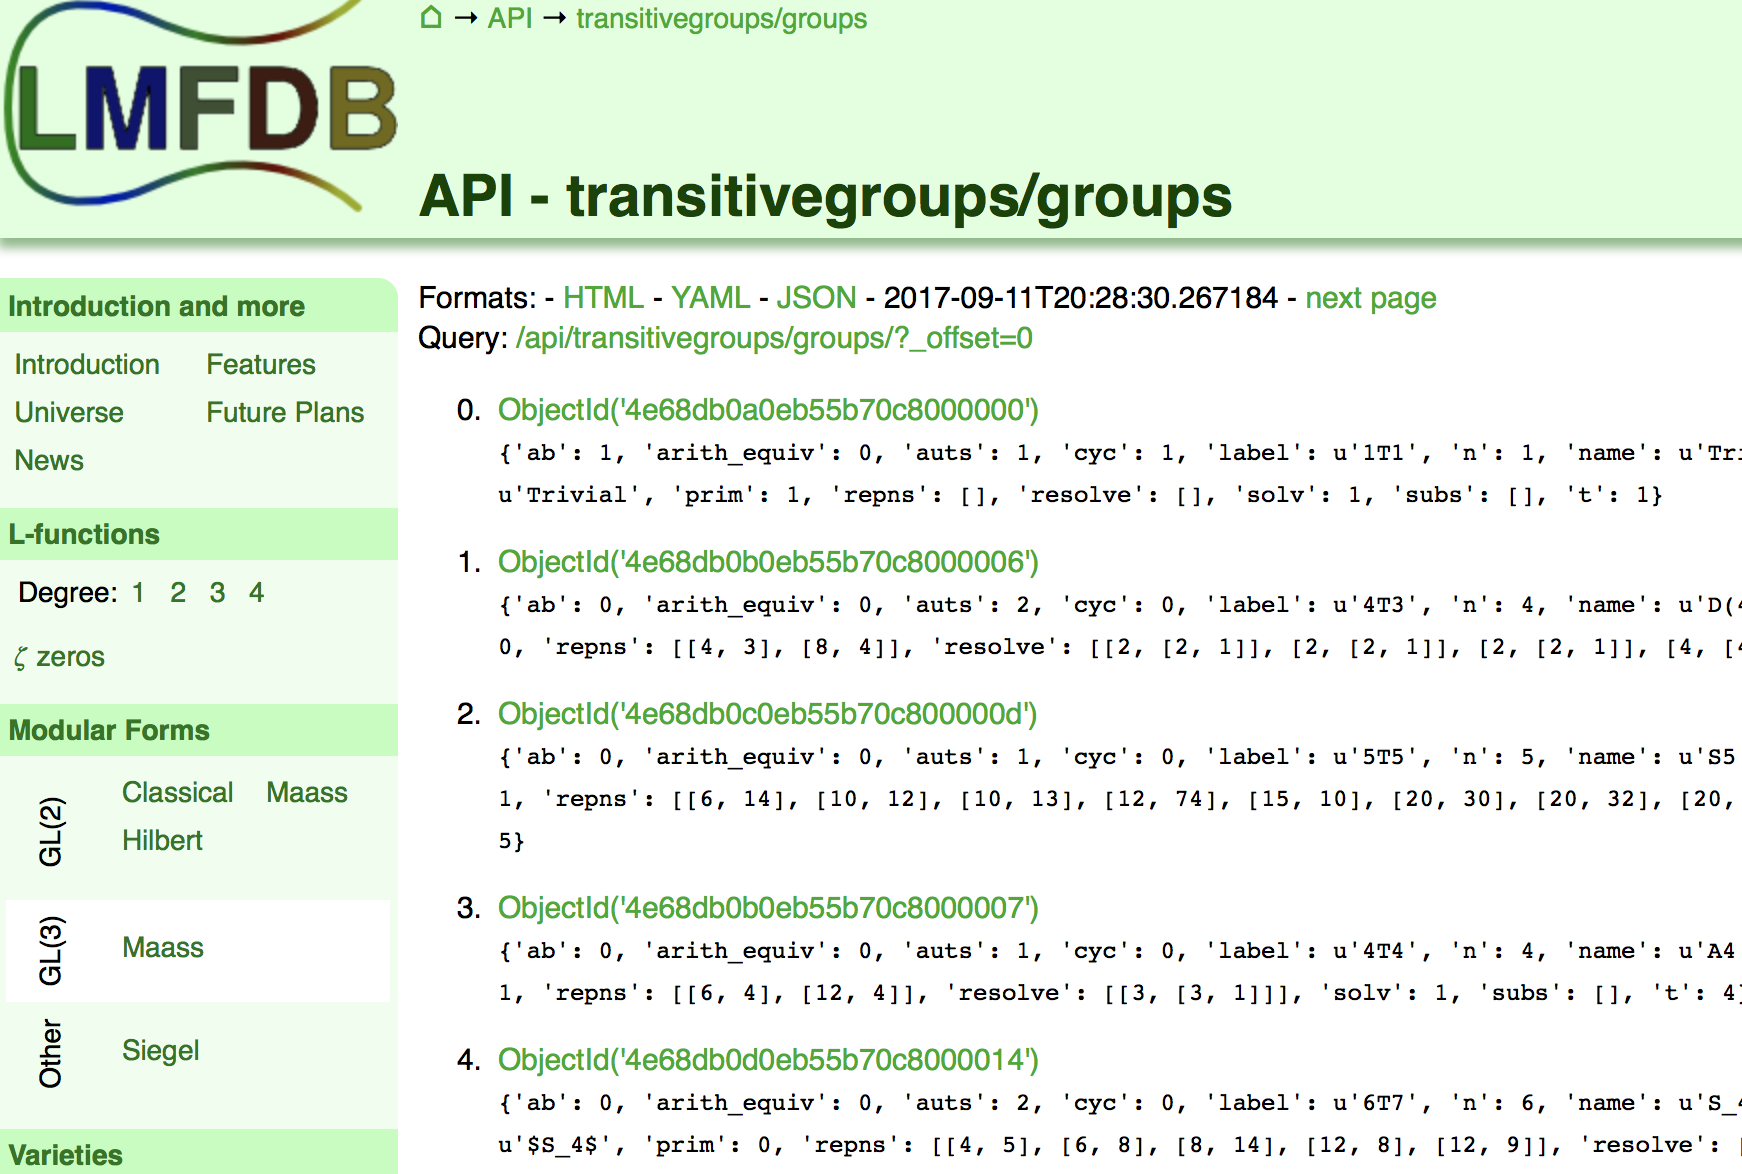
\includegraphics[width=0.7\textwidth]{APIScreenshot.png}
  \caption[The Web-Interface for the \lmfdb API. ]{
    The Web-Interface for the \lmfdb API. 
  }
  \label{fig:apiscreenshot}
\end{wrapfigure}
As \lmfdb is is a mathematical knowledge base, one important use case is to find elliptic curves subject to specific criteria. 
Consider for example a mathematician that wants to find all abelian elliptic curves in \lmfdb. 
How can this be achieved using the \lmfdb API located at \cite{lmfdbapi}? 

Queries can be sent to the API by making appropriate GET requests. 
The \lmfdb API can present results in two different ways, either using a web-based interface or programmatically by returning a set of JSON objects. 
A screenshot of the former can be seen in Figure~\ref{fig:apiscreenshot}. 

Queries must be formulated in terms of the underlying MongoDB schema, are sub-database specific, and should consist of a set of key value pairs. 
To solve the example given here we need to send the key-value pair \identifier{commutative}$ = $ \identifier{true}, finding all elements for which the commutative property is true. 
However, these values need to be encoded to be understood by MongoDB. 
We need to realize that the \identifier{ab} key corresponds to the commutativity property, has boolean values, and that MongoDB encodes \inlinecode{true} as \inlinecode{1}, and \inlinecode{false} as \inlinecode{0} in this \lmfdb sub-database. 
This information can then be used to make a query by sending a request to \url{http://www.lmfdb.org/api/transitivegroups/groups/?ab=1}. 

In this example, each of the steps are relatively straightforward. 
In a general setting, e.g. when searching for all elliptic curves with a specific isogeny matrix, this not only requires a good familiarity with the mathematical background but also with the system internals of the particular \lmfdb sub-database; a skillset commonly found in neither research programmers nor average mathematicians.   

To summarize: while \lmfdb offers a programmable API for accessing its contents, the content API is at the MongoDB level, and not the level of mathematical objects. 
Our Diagnosis is that \lmfdb -- and most other mathematical knowledge databases -- suffer from a double impedance mismatch problem.
\begin{compactenum}[\bf {I}1]
\item \emph{human/computer impedance mismatch}: Humans have problems interacting with \lmfdb, since they must speak the system language instead \lmfdb speaking mathematics
\item \emph{computer/computer impedance mismatch}: mathematical computer systems cannot interoperate, since their system languages differ.
\end{compactenum}
The MitM approach we have presented in Section~\ref{sec:mmtmitm}, we can solve both problems at the same time by lifting the communication to the level of \ommt-encoded MitM objects, which both MitM-compatible software systems and humans speak -- this is the central assumption of the MitM approach.
%%% Local Variables:
%%% mode: latex
%%% TeX-master: "paper"
%%% End:

%  LocalWords:  sec:sota lmfdb lmfdb lstlisting json ainvs iwp0 2adic_gens isogeny_matrix
%  LocalWords:  tamagawa_product 2adic_index anlist 4f71d4304d47869291435e6e vspace emph
%  LocalWords:  fig:lmfdbexample isogeny includegraphics textwidth fig:apiscreenshot
%  LocalWords:  centering summarize sec:mmtmitm ommt-encoded 4f71d4304d47869291435e6e
%  LocalWords:  serialization wrapfigure
